\documentclass[conference]{IEEEtran}
\IEEEoverridecommandlockouts
% The preceding line is only needed to identify funding in the first footnote. If that is unneeded, please comment it out.
\usepackage{cite}
\usepackage{amsmath,amssymb,amsfonts}
\usepackage{algorithmic}
\usepackage{graphicx}
\usepackage{textcomp}
\usepackage{xcolor}
%
\usepackage{booktabs}
\usepackage{multirow}
\usepackage{algorithm}
%
\def\BibTeX{{\rm B\kern-.05em{\sc i\kern-.025em b}\kern-.08em
    T\kern-.1667em\lower.7ex\hbox{E}\kern-.125emX}}
\begin{document}

\title{Toward An Efficient Cache Management Framework}

\author{\IEEEauthorblockN{1\textsuperscript{st} Xuewei Niu}
\IEEEauthorblockA{\textit{School of Information Science and Engineering,} \\ \textit{University of Jinan} \\
Jinan 250022, China \\
a@niuxuewei.com}
\and
\IEEEauthorblockN{2\textsuperscript{nd} Kun Ma*}
\IEEEauthorblockA{\textit{Shandong Provincial Key Laboratory of}\\ \textit{Network Based Intelligent Computing,}\\
\textit{University of Jinan} \\
Jinan 250022, China \\
ise\_mak@ujn.edu.cn}
}

\maketitle

\begin{abstract}
Nowadays, many companies used the cache clusters to reduce the pressure when network traffic peak is coming. For general cache manage framework, it might cause query bottleneck and lead to the availability of services. Therefore, building an efficient cache manage framework is meaningful. In this paper, we purpose an efficient cache management framework, Aspect-oriented Cache Auto Load Framework with Annotation(called ACALFA for short). There are some features for improving performance. Auto load allows the hot-spot keys to be preserved in the memory. And load wait allows the data are obtained by a leader who is selected by the framework for the same requests. The result of experiments indicated that our approach is nearly 25\% faster than other cache frameworks in the scenario that data size is enormous and concurrency is very high.
\end{abstract}

\begin{IEEEkeywords}
Data Cache, Auto Load, Load Wait, Cache Batch Deletion
\end{IEEEkeywords}

\section{Introduction}
\label{Introduction}

\subsection{Background}
Essential features of big data are Volume, Variety and Velocity (3V). It also brings significant challenges for data access and storage \cite{kaisler2013big}. For example, Facebook has become a producer of big data, using the integration of MySQL and NoSQL \cite{tang2015ripq}. In the case of high concurrency, these systems face cache penetration \cite{nishtala2013scaling}.

Cache is a collection of data duplicating original values stored in memory, usually for easier access. Moreover, it can reduce the server response time efficiently \cite{ma2017segment}. There are many ways to implement the cache, such as the cache based on browser, the cache based on CDN \cite{davis2013java} and the cache based on applications \cite{wu2011characterization}. Relative Database Management Systems (RDBMSs) combined with the NoSQL databases is the primary solution for the dynamic data, RDBMSs are used for data persistence, in-memory NoSQL databases are used for caching \cite{ma2017stream}.

There are a lot of cache management systems, but they all have some shortcomings. Firstly, for the data that will be accessed frequently or need a long time to process, the general expired strategy that caches have a fixed expired time rather than lurk in the memory constantly might lead to the server instability \cite{ma2017column}. Secondly, if cache miss, there are many requests for the same data in the high-concurrent scenario. RDBMSs need to handle those duplicate requests directly. These inefficient works bring about the service not available eventually. Thirdly, if perform update operation, cache deletion is a way to avoid the inconsistency, but there isn't a effective measure to implement it when the architecture become complex.

\subsection{Contributions}
In this paper, we propose an efficient cache management. Contributions of our framework are using the auto load and load wait mechanism for cutting down the read back of source, and using the hfield for reducing the cache deletion complexity.

\begin{itemize}
  \item Auto load can implement hot-spot data pre-loading. The cache work because the data can be obtained from memory and cut down the read back of source. To further reduce the read back of source, we can make the hot-spot data lurk in memory constantly and update it regularly. Moreover, the data that need to a long time to process also benefit from this strategy, system can load them before peak coming.
  \item Load wait can reduce the server pressure when load data from database. Once the cache miss, there are many requests flowing into the database, but for the same data. Load wait strategy select a leader to request the data, others wait until the data are provided by the leader.
  \item Cache batch deletions. It is inevitable that it leads the inconsistency of physical database and cache data. It is difficult to restore the key of the related cache by programs if the query statement is involved only. Therefore, the precise cache batch deletions are proposed.
\end{itemize}

\subsection{Organization}
The remainder of the paper is organized as follows. The current work of cache framework is discussed in Section \ref{RelatedWork}. In Section \ref{Framework}, an efficient cache framework is proposed. Some cache storage strategies, such as auto load, load wait, are introduced. In Section \ref{expriments}, the response time, resource consumption and pressure test experiments show that our framework are effective and efficient. Brief conclusions and future research directions are outlined in the last section.

\section{Related Work}
\label{RelatedWork}
Caching of data with weak consistency can achieve transparency. Typically, the cache content is periodically refreshed. There are different levels for caching performance, namely the browser cache \cite{davison2001web}, proxy cache \cite{uruburo2014methodology}, Content Delivery Network (CDN) cache \cite{vakali2003content}, and server level cache \cite{ma2017column}. Browser cache is closest to the end user and can speed up page loads by storing the static files, such as a single page, on user's local storage media \cite{mookerjee2002analysis}. CachePortal \cite{candan2001enabling} relies on timestamps and HTTP logs to conservatively determine which pages to invalidate. It has a unique form of weak, time-lagged consistency. Proxy caches are situated at network access points for web users \cite{uruburo2014methodology}. Consequently, proxy caches can store documents and directly serve requests for them in the network, thereby avoiding repeated traffic to web servers. CDN is similar to proxy caching \cite{vakali2003content}. But the difference is that the servers of CDN are distributed around the users, data is obtained from the server with least delay. The disadvantage of CDN cache is that excessive consumption of resources due to continuous analysis. Proxy cache and CDN solves the problem of the local cache cannot be shared. Although some of these products implement dynamic page cache, the effects are not good. In particular, server data processing efficiency is not effectively improved. Therefore, the present mainstream of cache is server level cache.

The combination of RDBMSs and in-memory NoSQL is the mainstream architecture of server cache. Several solusions are proposed such as Redis \cite{zawodny2009redis}, Memcached \cite{hafeez2017realizing}, and EhCache. RDBMSs are used to persist data, and in-memory databases are used to store high-frequency data \cite {ma2017column}. Redis performs better for high concurrency and memory consumption. As an improvement, Memcache pool is used to duplicate high-frequency data into a dedicated data pool by cache access frequency and cache expired cost \cite{nishtala2013scaling}. This feature is achieved by the time of the cache analysis by some dedicated servers.

\section{ACALFA: An Efficient Cache Management Framework}
\label{Framework}

\subsection{Architecture}

\begin{figure} [htb]
    \centering
    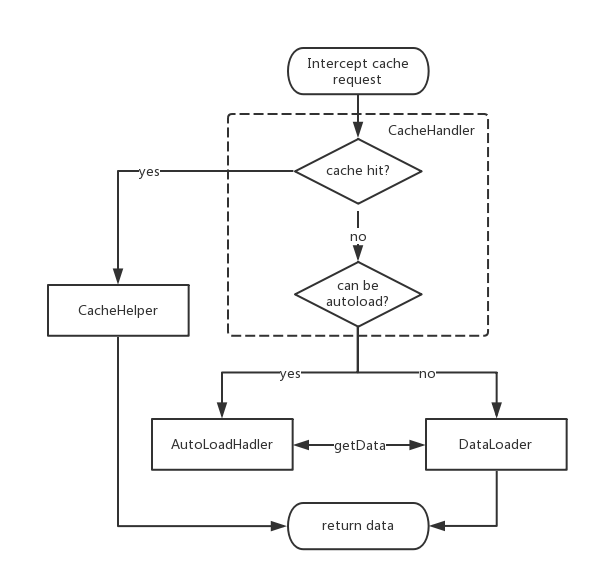
\includegraphics[width=1\linewidth]{img/architecture.png}
    \caption{Executive process of ACALFA}
    \label{Executive process of ACALFA}
\end{figure}

There are 4 main components to implement it:

\begin{itemize}
    \item CacheHandler: It is charged with process control rather than specific business. It parses cache configurations - are loaded from $@Cache$ Annotation - by expression parser. The crucial cache configurations are as follow:
    \begin{itemize}
        \item CacheKey is a cache identification expression, which can generate cache key dynamically according to the parameters.
        \item ExpireTime is a value to set up the cache expire time, the default value is 120(s).
        \item IsCacheable is a expression that return true or false to determined whether the cache can be cachable.
        \item IsAutoload is a expression that return true or false to determined whether the cache should be auto loading.
    \end{itemize}
    \item AutoLoadHandler: It, maintaining multiple internal tasks and queues, is seen as auto load executor. The cache that is going to expire update by loading asynchronous. The details will be described in following section.
    \item DataLoader: It works with DAO(Data Access Object) for fetching data from database and prevents the excessive traffic from coming into database. Therefore, the load wait strategy is implemented in this component.
    \item CacheHelper: It encapsulates functions of operating cache, such as get, set.
\end{itemize}

Figure \ref{Executive process of ACALFA} gives the simplified architecture of our proposed cache management framework that is used for reducing the read back of sources. When interceptor intercepts cache request, CacheHelper start to handle it on the basic of cache configurations. First of all, CacheHandler should judge the cache state, cache hit, indicates that cache of corresponding data exists in the cache, or cache miss, means the system should fetch data from physical database, by CacheKey. And then, CacheHandler should decide whether the cache need to be added to auto load queue according to the IsAutoload and IsCacheable. Finally, the query data need be synchronized to the cache asynchronously. If the IsCacheable is true, the data will be saved to cache and return, if not, only return.

\subsection{A Pre-Loading Strategy: Auto Load}

\begin{figure*} [htb]
    \centering
    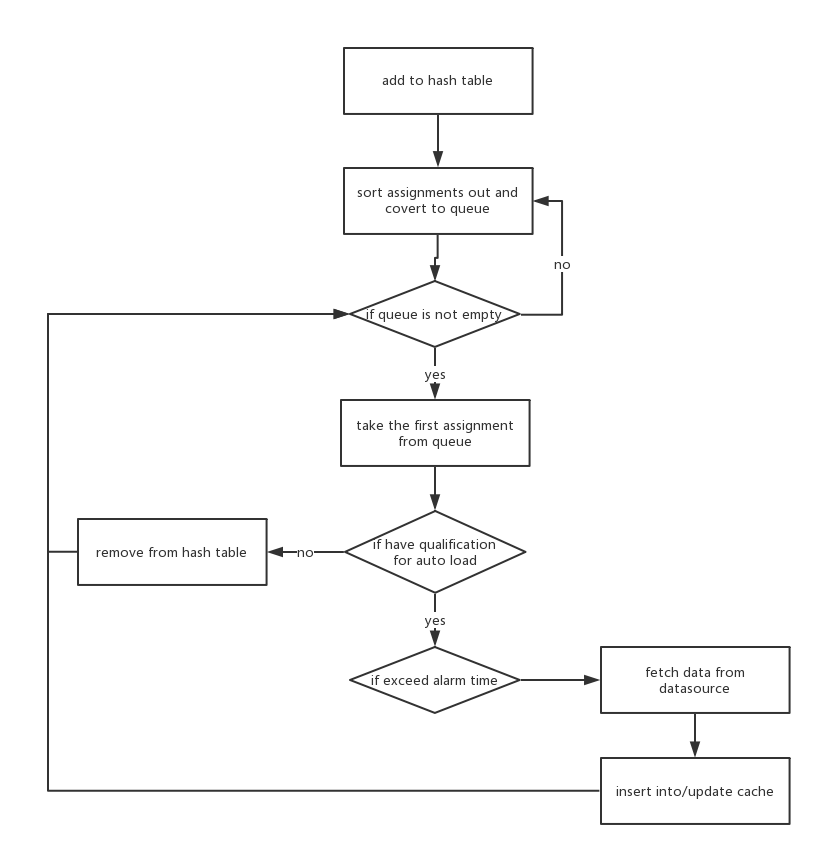
\includegraphics[width=0.9\linewidth]{img/autoload.png}
    \caption{Executive process of auto load}
    \label{process}
\end{figure*}

Generally, each cache have its own expired time, which it's not suitable for high-frequent cache or time-consuming data in in-memory cache. Once expired, the system has to fetch those data from data source, which may consume lots of resources and make response slow. Therefore, those types of data should reside in the memory until they don't take too many resources when fetching them.

Figure \ref{process} shows the executive process of auto load. $hashTable$, which providing a method called $putIfAbsent$ to avoid duplicate tasks and controlling the number of auto load tasks, is a storage for auto load assignments. $taskQueue$ is taken from $hashTable$ by a unified strategy, like LRU. In distributed scenario, the standardized sequence of tasks help the system reduce the read back of source, because others can fetch data from cache rather than database after first server loaded. Auto load, however, is a double-edged, the system may become unstable if the amount of auto load tasks were too much or update frequency were too high. Accordingly, a strict inspection should be applied. We assume that $t_n$(ms) is current time, $t_{fr}$(ms) is the first request time, $t_{lr}$(ms) is last request time,  $t_a$(ms) is the average of fetching time, $c$ is the times of cache usage, $t_{to}$ is a preset parameter determining cache time out. There are three main aspects as follow:

\begin{itemize}
    \item Remove if the targeting cache is not requested for a long time. The time of not be requested is get from $t_{nr} = t_n - t_{lr}$, if $t_{nr} > t_{to}$, the task will be discarded.
    \item Remove if efficiency of fetching data from database is high. This may be confused. The intention of auto load is pre-load the data that cost a lot of time and resources and be accessed frequently. Hence, the data that obtaining efficiency is high should not occupy the space of auto load. The standard of determination is $c > 100$ and $t_a < 10$.
    \item Remove if usage rate is low. If the cache, which is requested only once within the preset timeout, were added to auto load queue, that will go against the purposes of auto load. Therefore, only removing the task that the targeting cache is not requested for a long time is not enough. The usage rate can be get from $r = \frac{c}{\frac{t_n - t_{fr}}{3600000}}$, the meaning of $r$ is how much the cache is requested per hours. If the task has been running for more than 1 hour and the average loading time is less than 1000 ms and $r$ is less than 60, the task will be removed.
\end{itemize}{}

The last part of auto load is when to refresh the cache. As a pre-loading schema, the cache should be refreshed before expired. For this reason, setting alarm time is valuable. Experiments prove that the default alarm time should be set $t_e - 120$ if $t_e \geq 600$ or $t_e - 60$ if $t_e < 600$, which $t_e$ is a preset parameter determining cache expired time.

\subsection{Load Wait Strategy}

\begin{figure} [htb]
    \centering
    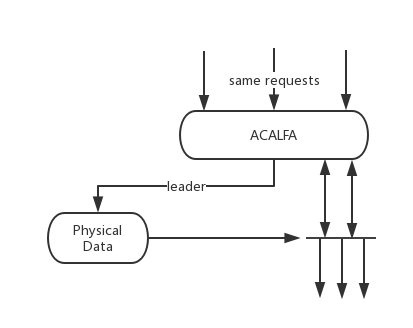
\includegraphics[width=0.8\linewidth]{img/load-wait-strategy.png}
    \caption{Process of load waiting strategy.}
    \label{load_wait_strategy}
\end{figure}

Load wait strategy works when the cache missed. Once hot-spot data miss and there are mass of requests flowing into database within a very short period time. After analyzed those requests, we found the proliferation of requests are same and can be optimized for alleviating the pressure on the database. The principle is to select a leader to fetch data from database, others, requesting for data with the same key, will be suspended until the leader processed. Figure \ref{load_wait_strategy} shows the process of load waiting strategy.

The framework identify the same requests by the cacheKey, which is a unique identification for the data. Processing is a hash map storing the different processing requests. A request want to fetch the data from database, DataLoader will search whether the same request is being processed. The framework try to get request from Processing hash map by cacheKey. If the result is null, it indicates that the request is a new request. In the concurrency, there are mass of the requests, the framework will select the first request as a leader to fetch data from physical data, others are waiting until the leader notify them and bring the data back. The specific load waiting strategy algorithm is as Algorithm \ref{loadwaitingalg}.

\begin{algorithm}
\caption{Load waiting strategy algorithm \textit{loadwaiting}}
\label{loadwaitingalg}

\algsetup{linenosize=\tiny}
\scriptsize

\begin{algorithmic}[1]
\REQUIRE ~~\\
  String $cacheKey$;\\
  Map $hashMap$;
\ENSURE ~~\\

\STATE Processing processing = hashMap.get(cacheKey);
\IF{processing == null}
\STATE Processing newProcessing = new Processing();
\STATE Processing \_processing = HashMap.putIfAbsent(cacheKey, newProcessing);
\IF{null != \_processing}
\STATE processing = \_processing
\ENDIF
\ENDIF

\IF{processing == null}
\STATE doRequest(newProcessing)
\STATE newProcessing.setFirstFinish(TRUE);
\STATE hashMap.remove(cacheKey);
\STATE newProcessing.notifyAll();
\ELSE
\STATE waitUntilLeaderGotData(processing);
\ENDIF


\RETURN

\medskip

\end{algorithmic}
\end{algorithm}

\subsection{Cache Batch Deletions}
It's difficult to restore or obtain the cache key that need to delete when the query statements are complex, active deletion will hardly complete. In order to manage that, "namespace + hfield + cachekey" schema is proposed. The cache is added string, indicating its namespace, before the cache key, aiming to address conflict in the cache cluster. For active deletion, the key point is that establish a hash table to store the caches that need to be removed together. "hfield" is to identify a unique hash table. Developers can design the deletion granularity on need basis. The process of cache batch deletions is ACALFA intercepts the delete request and inspect whether hfield is set. If hfield is set, ACALFA will delete all the cache that store in corresponding hash table. If not, ACALFA will only delete that cache.

\section{Experiments}
\label{expriments}

\subsection{Experiment Setup}
Three experiments are designed to illustrate the ACALFA performance in high-concurrency scenario. The metrics are response time, resource consumption and stability. Response time is for validating the optimization of auto load, especially for time-consuming tasks and high-frequent business. Resource consumption is for validating the load wait performance when handling the same requests. Stability testing uses multiple threads to access applications simultaneously to simulate high concurrency. The server with ACALFA is an Intel Core i7 @ 3.40GHz CPU, 16GB memory, and 100Mbps bandwidth, and this server runs a 64-bit Windows 10 with a Java 1.8 64-bit server JVM. Another server with MySQL database runs on Ali ECS Cloud Server: 2 core 2.60GHz Intel Xeon E5-2650 CPU machines with 4 GB RAM, 40GB SSD and 100 Mbps Ethernet. The system is CentOS 6.8 x64. Spring Cache, a well-known cache management framework at j2ee, will be compared with ACALFA for performance. The dataset, the structure is shown in Table \ref{VTS}, is selected 4,000 records randomly from a voting system.

\begin{table*}[htb]
\begin{center}
 \caption{\label{VTS}Voting Table Structure.}
 \begin{tabular}{lll}
 \toprule
    Field & Type & Description\\
 \midrule
    id & INT & primary key\\
    candidate\_id & INT & candidate identification\\
    voter\_id & INT & voter identification\\
    score & INT & candidate scores between 1, 100\\
\bottomrule
 \end{tabular}
\end{center}
\end{table*}

\subsection{Response Time}

We set up six experiments to test the ACALFA effect. Cache expired time we set was 120s and enabled auto load and load wait for ACALFA. Exp1, exp3 and exp5 used ACALFA, on the contrary, others used Spring Cache. The experiment sets are as follow:

\begin{itemize}
    \item Exp1 \& Exp2: The resources that will be requested were not in cache. Therefore, the frameworks should fetch data from database.
    \item Exp3 \& Exp4: The response time when cache hit.
    \item Exp5 \& Exp6: After exp1 and exp2 120s, in other words, cache expired, we send requests again for validating the effect of auto load.
\end{itemize}

\begin{figure} [htb]
    \centering
    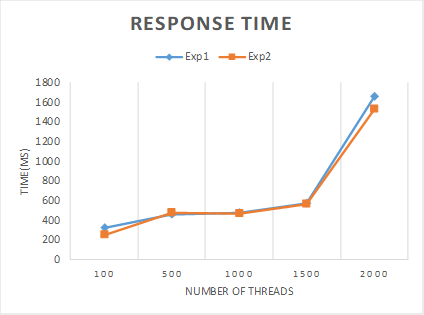
\includegraphics[width=1\linewidth]{img/exp1-2.png}
    \caption{Response time of Exp1 and Exp2}
    \label{exp1-2}
\end{figure}

\begin{figure} [htb]
    \centering
    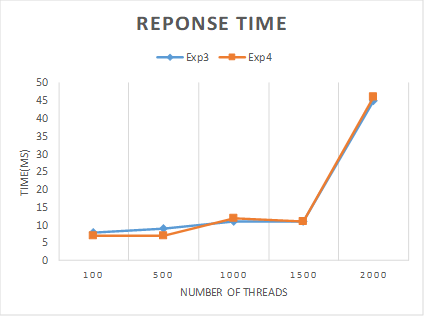
\includegraphics[width=1\linewidth]{img/exp3-4.png}
    \caption{Response time of Exp1 and Exp2}
    \label{exp3-4}
\end{figure}

\begin{figure} [htb]
    \centering
    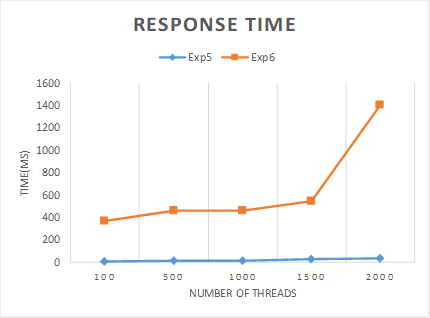
\includegraphics[width=1\linewidth]{img/exp5-6.png}
    \caption{Response time of Exp1 and Exp2}
    \label{exp5-6}
\end{figure}

We use the 90th percentile response time for performance measurement. Figure \ref{exp1-2} and figure \ref{exp3-4} shows the response time is increasing with the increase of number of threads. The performance of two cache management systems when cache miss or cache hit is same roughly. Figure \ref{exp5-6}, however, shows vast difference between ACALFA with auto load and Spring Cache. The reason is obviously: ACALFA will reload data when the cache is going to expire, but Spring Cache can't. According to this range of experiments, we found auto load is suited to the hot-spot data and has better cache effects for the more time-consuming or more frequent data.

\subsection{Resource Consumption}

Resource consumption experiment is set for validating the load wait performance. Therefore, the cache is disabled and the query statement is changed to join two tables for increasing cpu usage. There are 30 threads and request 10 times repeatedly. The CPU usage is shown in figure \ref{resource}. From results, CPU usage of non-load-wait lasted for a long time in 100\%. However, ACALFA selected a leader to fetch data in each round of request to reduce the CPU consumption. According to the results, we found wait-load strategy is effective in cache miss situation. Coordinate with auto-load, ACALFA can deal with complex and high-concurrent scenario well.

\begin{figure} [htb]
    \centering
    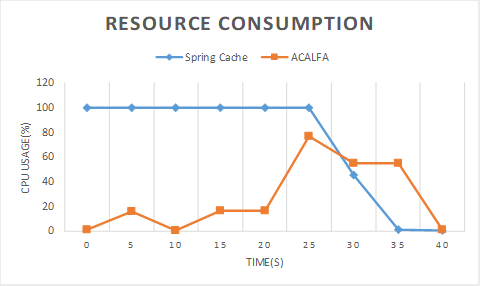
\includegraphics[width=1\linewidth]{img/resource.png}
    \caption{CPU usage of performing the select statement}
    \label{resource}
\end{figure}

\subsection{Pressure Test}

 \begin{figure}
     \centering
     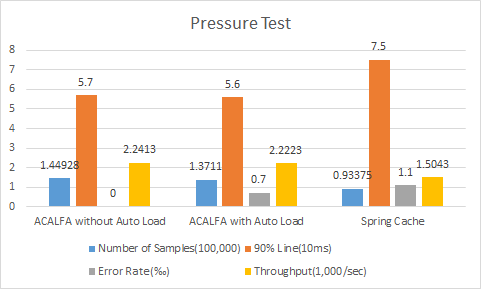
\includegraphics[width=1\linewidth]{img/pressuretest.png}
     \caption{Pressure with different methods}
     \label{pressuretest}
 \end{figure}

 The pressure test is getting access to a page repeatedly within one minute in order to test the stability of ACALFA in high concurrency. We used 100 threads to simulate 100 users for requesting the targeting page simultaneously. We can infer the system availability and response speed from the report. The query statement is same as resource consumption experiment. We can learn ACALFA response is 25\% faster than Spring Cache, processing speed is 48\% faster and stability has improved 36\% from above figure \ref{pressuretest}.

\section{Conclusions}
\label{Conclusions}
The purpose of a cache is to duplicate frequently accessed or important data in such a way that it can be accessed very fast and close to where it is needed. In the big data era, caching generally moves data from a low cost. This paper introduces ACALFA - an efficient cache management system. Several experiments are illustrated that our cache framework has a good effect on the complex business with high concurrency. In the future work, memory resource cost will be optimized to increase cache hit ratio.

\section*{Acknowledgment}
This work was supported by the National Natural Science Foundation of China (61772231 \& 61702217 \& 61702216), the Shandong Provincial Natural Science Foundation (ZR2017MF025 \& ZR2014FQ029), the Shandong Provincial Key R\&D Program of China (2015GGX106007 \& 2016ZDJS01A12 \& 2017CXGC0701 \& 2018CXGC0706), the Science and Technology Program of University of Jinan (XKY1734 \& XKY1828). Kun Ma is the corresponding author.

\bibliographystyle{IEEEtran}
\bibliography{mybibtex}

\end{document}
